\documentclass[article]{jss}\usepackage[]{graphicx}\usepackage[]{color}
%% maxwidth is the original width if it is less than linewidth
%% otherwise use linewidth (to make sure the graphics do not exceed the margin)
\makeatletter
\def\maxwidth{ %
  \ifdim\Gin@nat@width>\linewidth
    \linewidth
  \else
    \Gin@nat@width
  \fi
}
\makeatother

\definecolor{fgcolor}{rgb}{0.345, 0.345, 0.345}
\newcommand{\hlnum}[1]{\textcolor[rgb]{0.686,0.059,0.569}{#1}}%
\newcommand{\hlstr}[1]{\textcolor[rgb]{0.192,0.494,0.8}{#1}}%
\newcommand{\hlcom}[1]{\textcolor[rgb]{0.678,0.584,0.686}{\textit{#1}}}%
\newcommand{\hlopt}[1]{\textcolor[rgb]{0,0,0}{#1}}%
\newcommand{\hlstd}[1]{\textcolor[rgb]{0.345,0.345,0.345}{#1}}%
\newcommand{\hlkwa}[1]{\textcolor[rgb]{0.161,0.373,0.58}{\textbf{#1}}}%
\newcommand{\hlkwb}[1]{\textcolor[rgb]{0.69,0.353,0.396}{#1}}%
\newcommand{\hlkwc}[1]{\textcolor[rgb]{0.333,0.667,0.333}{#1}}%
\newcommand{\hlkwd}[1]{\textcolor[rgb]{0.737,0.353,0.396}{\textbf{#1}}}%
\let\hlipl\hlkwb

\usepackage{framed}
\makeatletter
\newenvironment{kframe}{%
 \def\at@end@of@kframe{}%
 \ifinner\ifhmode%
  \def\at@end@of@kframe{\end{minipage}}%
  \begin{minipage}{\columnwidth}%
 \fi\fi%
 \def\FrameCommand##1{\hskip\@totalleftmargin \hskip-\fboxsep
 \colorbox{shadecolor}{##1}\hskip-\fboxsep
     % There is no \\@totalrightmargin, so:
     \hskip-\linewidth \hskip-\@totalleftmargin \hskip\columnwidth}%
 \MakeFramed {\advance\hsize-\width
   \@totalleftmargin\z@ \linewidth\hsize
   \@setminipage}}%
 {\par\unskip\endMakeFramed%
 \at@end@of@kframe}
\makeatother

\definecolor{shadecolor}{rgb}{.97, .97, .97}
\definecolor{messagecolor}{rgb}{0, 0, 0}
\definecolor{warningcolor}{rgb}{1, 0, 1}
\definecolor{errorcolor}{rgb}{1, 0, 0}
\newenvironment{knitrout}{}{} % an empty environment to be redefined in TeX

\usepackage{alltt}

%%%%%%%%%%%%%%%%%%%%%%%%%%%%%%
%% declarations for jss.cls %%%%%%%%%%%%%%%%%%%%%%%%%%%%%%%%%%%%%%%%%%
%%%%%%%%%%%%%%%%%%%%%%%%%%%%%%

%% almost as usual
\author{Steve Bronder\\ Columbia University}
\title{Time Series Methods in the R package \pkg{MLR}}

%% for pretty printing and a nice hypersummary also set:
\Plainauthor{Steve Bronder} %% comma-separated
\Plaintitle{Time Series Methods in the R package \pkg{mlr}} %% without formatting
\Shorttitle{\pkg{mlr}: Time Series Methods} %% a short title (if necessary)

%% an abstract and keywords
\Abstract{
  The MLR package is a unified interface for machine learning tasks such as classification, regression, cluster analysis, and survival analysis. \pkg{mlr} handles the data pipeline of pre-processing, resampling, model selection, model tuning, ensembling, and prediction. This paper details new methods for developing time series  models in the \pkg{mlr}. It includes Standard and novel tools such as auto-regressive and LambertW transform data generating processes, fixed and growing window cross validation, and forecasting models in the context of univariate and multivariate time series. Examples from forecasting competitions will be given in order to demonstrate the benefits of a unified framework for machine learning and time series.
}
\Keywords{time series, model building, tuning parameters, \proglang{R}}
\Plainkeywords{time series, model building, tuning parameters, R} %% without formatting
%% at least one keyword must be supplied

%% publication information
%% NOTE: Typically, this can be left commented and will be filled out by the technical editor
%% \Volume{50}
%% \Issue{}
%% \Month{June}
%% \Year{2016}
%% \Submitdate{2012-06-04}
%% \Acceptdate{2012-06-04}

%% The address of (at least) one author should be given
%% in the following format:
\Address{
  Steve Bronder\\
  Quantitative Methods in the Social Sciences\\
  Columbia University in the City of New York\\
International Affairs Building, MC3355\\
420 W 118th St, Suite 807 \\
New York, NY 10027\\
  E-mail: \email{sab2287@columbia.edu}\\
  URL: \url{insert.url}
}
%% It is also possible to add a telephone and fax number
%% before the e-mail in the following format:
%% Telephone: +43/512/507-7103
%% Fax: +43/512/507-2851

%% for those who use Sweave please include the following line (with % symbols):
%\usepackage{Sweave}

%% end of declarations %%%%%%%%%%%%%%%%%%%%%%%%%%%%%%%%%%%%%%%%%%%%%%%
\IfFileExists{upquote.sty}{\usepackage{upquote}}{}
\begin{document}

%% include your article here, just as usual
%% Note that you should use the \pkg{}, \proglang{} and \code{} commands.

\section{Introduction}

There has been a rapid developement in time series methods over the last 25 years ~\cite{Hyndman25}. Time series models have not only become more common, but more complex. The \proglang{R} language ~\cite{Rbase} has a large task view with many packages available for forecasting and time series methods. However, without a standard framework, many packages have their own sub-culture of style, syntax, and output. The \pkg{mlr} ~\cite{mlr} package, short for Machine Learning in R, works to give a strong syntatic framework for the modeling pipeline. By automating many of the standard tools in machine learning such as preprocessing and cross validation, \pkg{mlr} reduces error in the modeling process that is derived from the user. 

While there are some time series methods available in the \pkg{caret} ~\cite{caret}, development of forecasting models in \pkg{caret} is difficult due to computational constraints and design choices. The highly modular structure of \pkg{mlr} makes it the best choice for implementing time series methods and models. This paper will show how using \pkg{mlr}'s strong syntatic structure allows for time series packages such as \pkg{forecast} ~\cite{HyndForecast} and \pkg{rugarch} ~\cite{rugarch} to use machine learning methedologies such as automated parameter tuning, data preprocessing, model blending, cross validation, performance evaluation, and parallel processing techniques for decreasing model build time.

\section{Forecasting Example with the M4 Competition}

Professional forecasters attempt to predict the future of a series based on its past values. Forecasting can be used in a wide range of tasks including forecasting stock prices, ~\cite{GRANGER19923}, weather patterns ~\cite{MurphymeteoForecast}, international conficts ~\cite{Chadefaux01012014}, and earthquakes ~\cite{earthquakeYegu}. In order to evaluate \pkg{mlr}'s forecasting framework we need a large set of possible time series to make sure our methods generalize well.\footnote{Very goofy sentence need to fix}
The Makridakis competitions ~\cite{Makridakis2000451} are forecasting challenges organized by the International Institute of Forecasters and led by Spyros Makridakis to evaluate and compare the accuracy of forecasting methods. The most recent of the competitions, the M4 competition, contains 10,000 time series on a yearly, quarterly, monthly, and daily frequency and areas such as finance, macroeconomics, microeconomics, and industry. For our purposes we will look at two particular daily financial series, one with 9136 observations from April 10th, 1971 to April 13th, 1996 and another with 6742 observations from January 7th, 1981 to June 23rd, 1999. Each series has a forecasting of 328 and 242 periods into the future, respectively.

\begin{knitrout}
\definecolor{shadecolor}{rgb}{0.969, 0.969, 0.969}\color{fgcolor}

{\centering 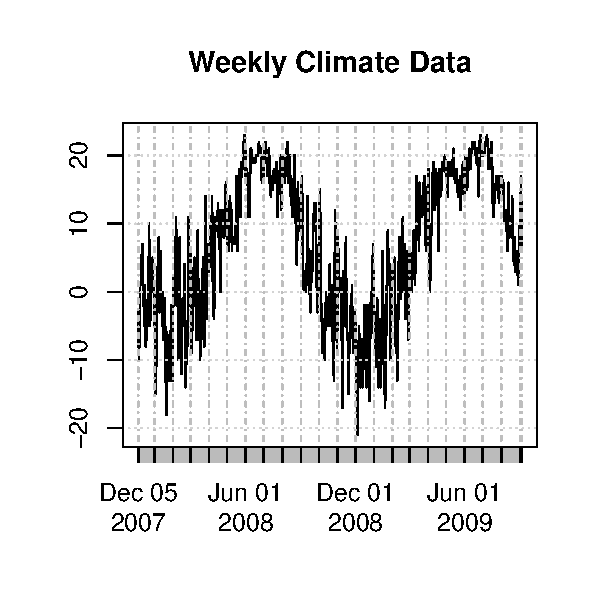
\includegraphics[width=\maxwidth]{figure/get_dat-1} 

}




{\centering 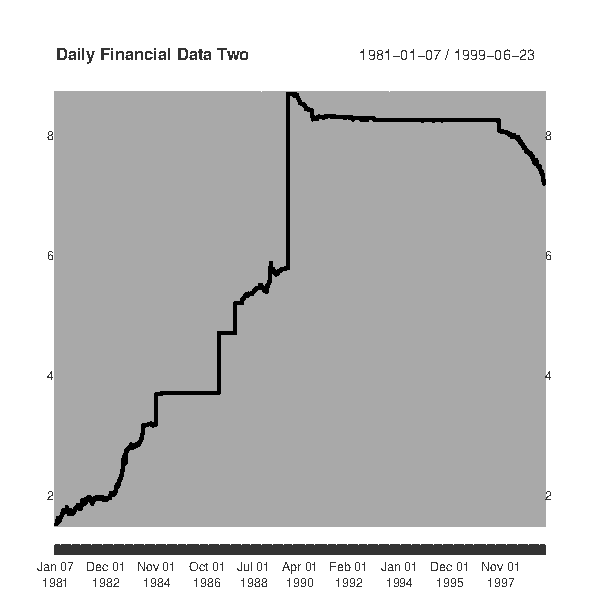
\includegraphics[width=\maxwidth]{figure/get_dat-2} 

}



\end{knitrout}

These two series were chosen for their large time features and stark contrast.\footnote{I think it would be better to just use one series for examples, and actually train / test over all of M4 later} Our data set should be large enough that the tuning method can take multiple windows of the data. Some series in M4 only contain 12 observations, which is not enough data to accurately train a model. These two time series were chosen as they are the two largest ones in the M4 competitions data set. We can see figure one is what most people imagine when they think of a time series. Figure two shows a series which appears to have a sort of step feature. The stark difference between the time process of the two series will allow us to investigate whether the methods in \pkg{mlr}'s forecasting framework can find the appropriate model. The data can be found in the package \pkg{M4comp} ~\cite{m4comp} under sets `M4[28]` and `M4[29]. 

\section{Forecasting Tasks}

\pkg{mlr} provides uses the S3 object system to clearly define a predictive modeling task. Tasks contain the data and other relevant information such as the task id and which variable you are targeting for supervised learning problems. Forecasting tasks are handled in \pkg{mlr} by the function \code{makeForecastRegrTask()}. The forecasting task inherets from \code{makeRegrTask()}, but has two noticable differences in parameters.

\begin{itemize}
\item[data:] Instead of a data frame, an xts object from \pkg{xts} ~\cite{xts} containing the time series.
\item[frequency:] An integer with the number of periods your time series contains. For example, daily data with a weekly periodicity has a frequency of 7 while daily data with a yearly frequency have a frequency of 365.
\end{itemize}

\begin{knitrout}
\definecolor{shadecolor}{rgb}{0.969, 0.969, 0.969}\color{fgcolor}\begin{kframe}
\begin{alltt}
\hlkwd{library}\hlstd{(mlr)}
\end{alltt}


{\ttfamily\noindent\itshape\color{messagecolor}{\#\# Loading required package: ParamHelpers}}\begin{alltt}
\hlstd{Fin.task1} \hlkwb{=} \hlkwd{makeForecastRegrTask}\hlstd{(}\hlkwc{id} \hlstd{=} \hlstr{"M4 Finance Data One"}\hlstd{,}
                                 \hlkwc{data} \hlstd{= m4Train1,}
                                 \hlkwc{target} \hlstd{=} \hlstr{"target_var"}\hlstd{)}
\hlstd{Fin.task1}
\end{alltt}
\begin{verbatim}
## Task: M4 Finance Data One
## Type: regr
## Observations: 9136
## Dates:
##  Start: 1971-04-10 
##  End: 1996-04-13
## Frequency: 1
## Features:
## numerics  factors  ordered 
##        1        0        0 
## Missings: FALSE
## Has weights: FALSE
## Has blocking: FALSE
\end{verbatim}
\end{kframe}
\end{knitrout}

\section{Building a forecast learner}

The \code{makeLearner()} function provides a structured model building framework to the 7 forecasting models currently implimented in \pkg{mlr}. As an example, we will build a simple AutoRegressive Integrated Moving Average (ARIMA) model. The ARIMA model is of the form

\begin{equation}
y_t \sim \alpha + \beta_1 \Delta_k y_{t-1} ... \beta_n \Delta_k y_{t-n} + \phi_1 \epsilon_{t-1} + ... + \phi_n \epsilon_{t-n} + \epsilon_t
\end{equation}

\begin{equation}
y_t \sim \alpha + \sum_{i=1}^n \beta_i y_{t-i} + \sum_{i=1}^n \phi_i \epsilon_{t-i} +\epsilon_t
\end{equation}

In equation three, $\alpha$ is a constant, $\beta_n$ is the coefficient associated with the lagged observations of $y$ with $\Delta_k$ being the $k$th difference operator. The coefficient for the one step forecast error $\epsilon_{t-n}$ is $\phi_n$.


\section{Resampling with Time}

Overfitting models is one of the most common problems in prediction. Resampling schemes such as cross-validation, bootstrapping, etc. are common in machine learning. When their is a time component to the data, windowing schemes are necessary so that we correctly resample while still validating the time component of the model\footnote{crap}. Growing and fixed window resampling such as from ~\cite{hyndman2014forecasting} are now available in the \code{resampling()} function of \pkg{mlr}.



\begin{figure}[h]
\caption{Resampling with a window scheme as exampled by caret}
  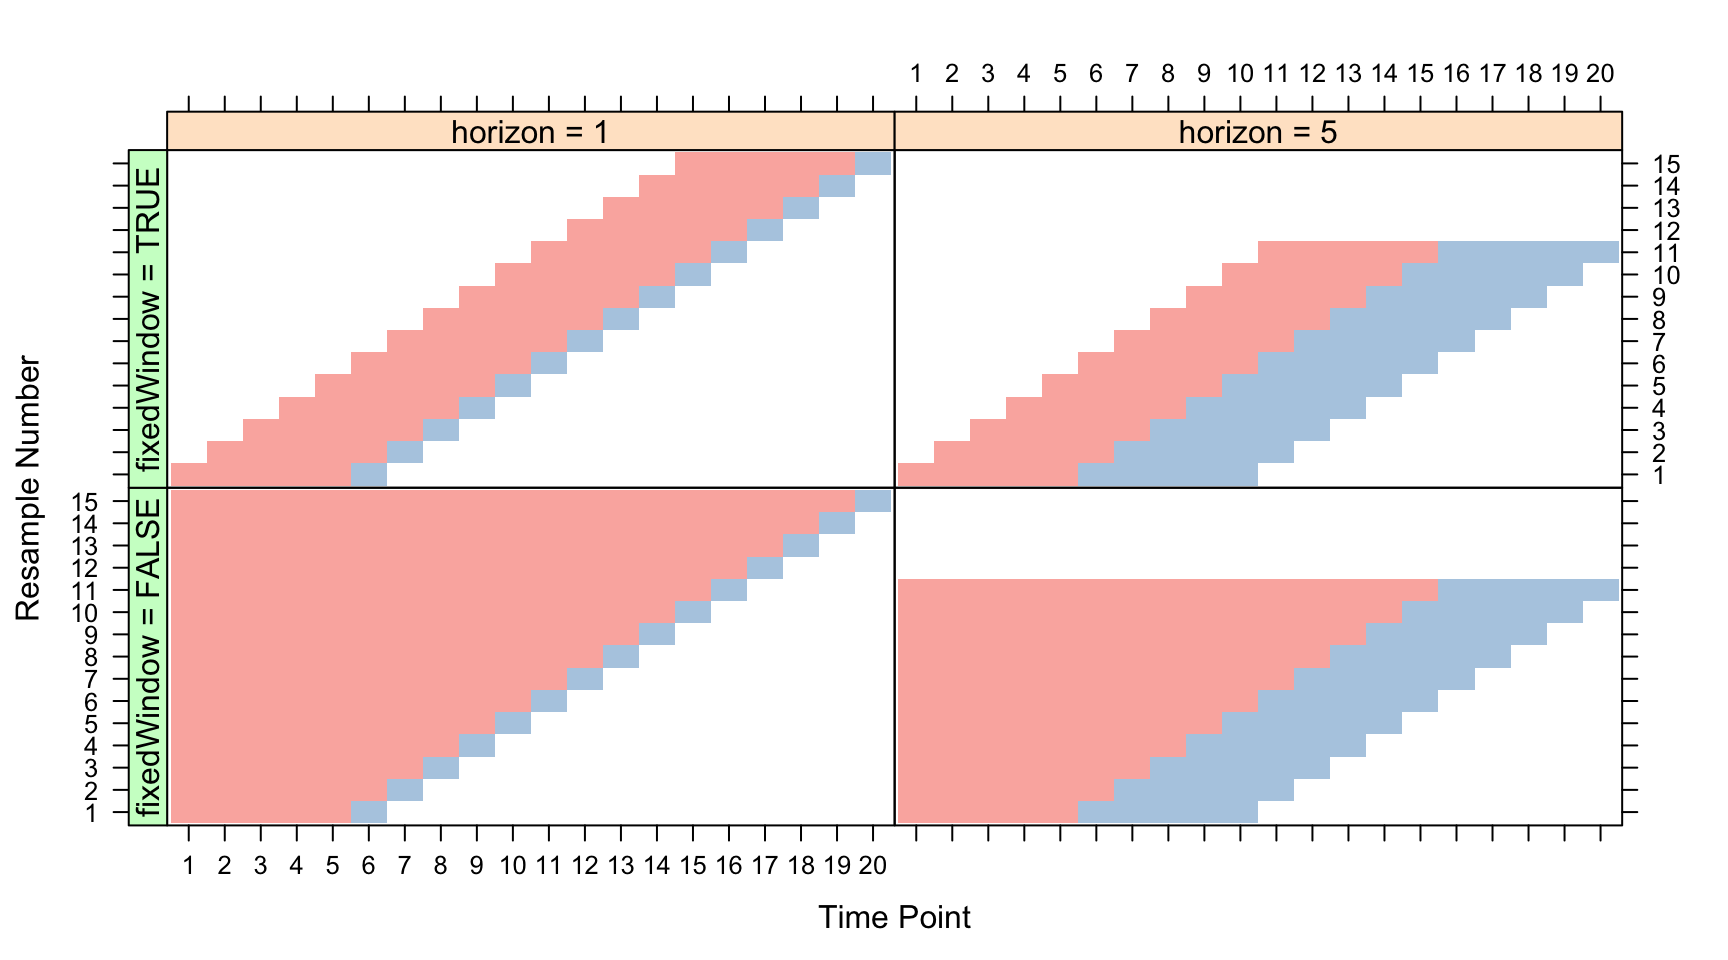
\includegraphics{windowing_pic_caret}
  \centering
\end{figure}
%% Note: If there is markup in \(sub)section, then it has to be escape as above.
\clearpage
\bibliographystyle{plainnat}
\bibliography{thesisbib}

\end{document}
